\section{Looking Under the Hood}
Our thorough experiments over a wide range of ABR techniques indicate that DASH/QUIC does not perform as well as it is supposed to. To explore this further, we perform a set of experiments to understand the issues with QUIC, which affect DASH-based video streaming.

\subsection{Does QUIC Perform Poorly in All Scenarios?}
One immediate question that might arise in this context is whether the observed performance drops are generic for QUIC, or whether certain features of QUIC affect the performance of DASH. With the similar network setup as discussed before, we compute the overall throughput and the response latency for TCP and QUIC over two different scenarios -- (a) downloading of large web-objects and (b) DASH video streaming. 
%The response latency is computed as the average latency between each request from the client to the server and the response back from the server to the client. We compare the performance between TCP and QUIC for the above two scenarios. 


\subsubsection{Performance during HTTP Object Downloads}
To see how the performances of TCP and QUIC fare during the download of HTTP web objects, we perform a set of experiments over the same network setup with emulated bandwidth control via {\tt Mahimahi} traffic shaper. We download HTTP web objects (HTML and data files) of predefined sizes (from $2$MB to $50$MB) for $40$ sequential HTTP requests in each session. We give a pause of $500$ms before requesting the next web object. We repeat each session three times for both TCP and QUIC. 


\begin{figure}[!ht]
	\captionsetup[subfigure]{}
	\begin{center}
		\subfloat[\label{fig:proofLargeFileThroughput}Throughput]{
			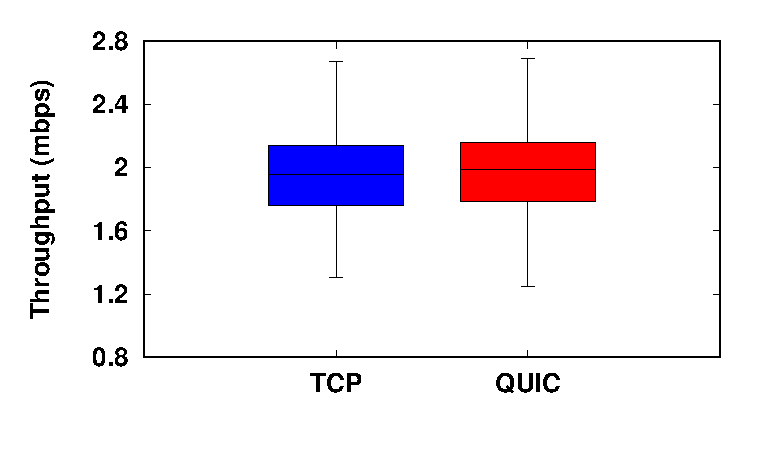
\includegraphics[width=.49\linewidth]{img/proof/largefile/throughput}
		}
		\subfloat[\label{fig:proofLargeFileWait}Response latency]{
			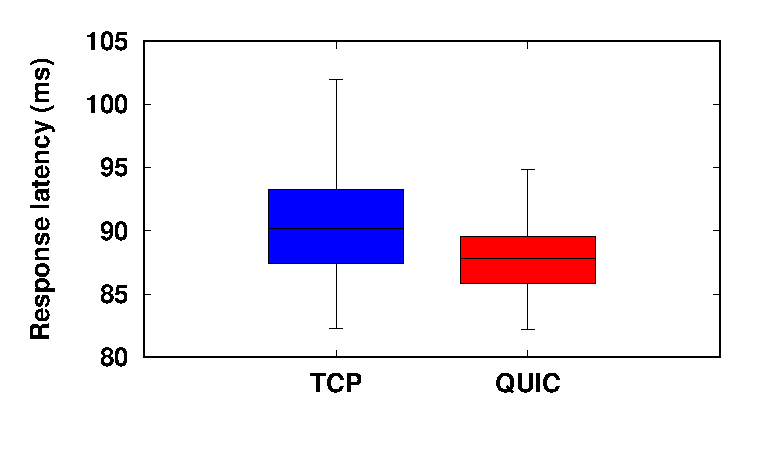
\includegraphics[width=.49\linewidth]{img/proof/largefile/wait}
		}
	\end{center}
	\caption{\label{fig:proofLargeFile}TCP and QUIC performance during HTTP web object download}
\end{figure}


%Fig.~\ref{fig:proofLargeFile} depicts the results from this experiment. In 
Fig.~\ref{fig:proofLargeFileThroughput} shows the distribution of throughput observed against each web object downloads, while Fig.~\ref{fig:proofLargeFileWait} indicates the response latency observed by each HTTP request. The throughput is computed as the object size divided by the download time where the download time is the time difference between the first and the last bytes received for that web object. The response latency is computed as the time between the initiation of the HTTP request and the time when the first byte of the response is received. From the figures, we see that the throughput is similar for HTTP/TCP and HTTP/QUIC. The response latency for HTTP/QUIC is slightly lower than HTTP/TCP. These experiments shows that QUIC performs better than TCP in terms of response latency which is an important QoE metric for web object downloads. 


\begin{figure}[!ht]
	\captionsetup[subfigure]{}
	\begin{center}
		\subfloat[\label{fig:proofCompThroughput} Throughput ]{
			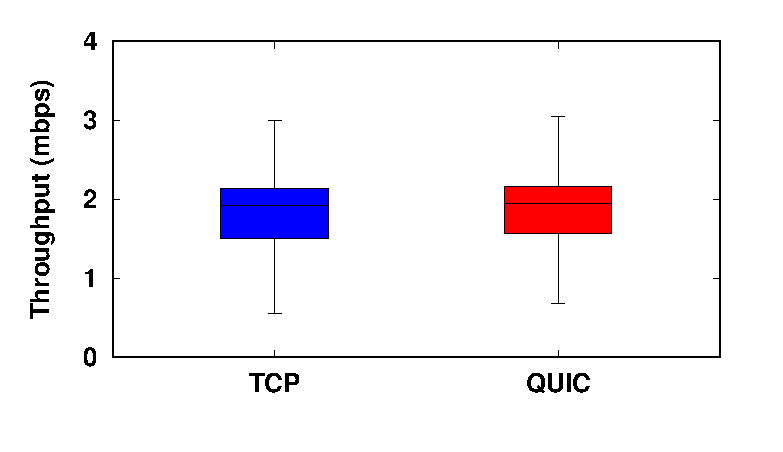
\includegraphics[width=.45\linewidth]{img/proof/comp/throughput}
		}
		\hfill
		\subfloat[\label{fig:proofCompWait} Response latency]{
			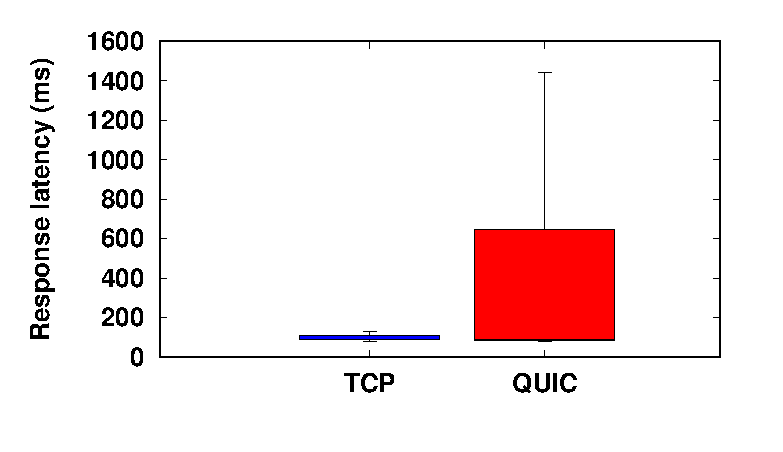
\includegraphics[width=.45\linewidth]{img/proof/comp/wait}
		}
	\end{center}
	\caption{\label{fig:dashcomp}TCP and QUIC performance during DASH video segment download}
\end{figure}


\subsubsection{Performance during Video Streaming}
Fig.~\ref{fig:proofCompThroughput} shows the distribution of the throughput observed during the video playback, combining the data from all the five ABR mechanisms. A statistical test also indicates that the difference between TCP and QUIC in terms of throughput is not significant. Interestingly, the predicted throughput during video streaming is one of the important metrics used by all the ABR mechanisms for deciding the optimal bitrate. Fig.~\ref{fig:proofCompWait} plots the distributions of the response latency, combining the videos from all the five ABR mechanisms. We have an interesting observation here -- although the difference in the median of the response latency for DASH/QUIC and DASH/TCP is not significant,  the upper quartile for the response latency of DASH/QUIC is significantly higher than the upper quartile of DASH/TCP. This indicates that with QUIC, the response latency sometime becomes very high -- this observation is opposite to what we have observed in Fig.~\ref{fig:proofLargeFileWait}. It can be noted that the throughput computation does not consider the response latency, rather it considers the time difference between the first and the last bytes received for a video segment. The ABR algorithms primarily select the bitrate based on the computed throughput for the last few video segments. If the computed throughput is high, the DASH client requests for the next video segment in an increased quality level. However, if the response latency is high, this segment may take longer time to reach the client, resulting in a rebuffering and subsequent drop in the quality levels for the next video segments. We do not see this problem for TCP, as the response latency correlates with the computed throughput; however, this correlation does not hold for QUIC. Next, we dig further to find out the reason behind the high response latency observed during the video streaming using QUIC. 
%From this experiment, the next question comes -- why is the response latency with QUIC very high sometimes?
%However, the throughput is computed based on the payload size and the download time only, which does not take care of the response time against each video request from the client to the server.  



%To understand the reason behind this, we plot the throughput observed by the DASH player in Fig.~\ref{fig:proofCompThroughput} as all the ABRs directly or indirectly depend on the observed throughput only. However, to our surprise, the observed throughput by the DASH player is comparably the same. So, we look into the DASH player source code to understand the throughput measurement technique. To measure the throughput, DASH player needs two components, the payload size and the download time. The DASH player measures the download time as the duration from the time it receives the first byte to the time receive the last byte. Although it is perfectly okay, it does not include the response latency that is the duration from the time it sends the request to the time it receives the first byte.
%}
%
%\blue{
%A DASH player fetches the video segments using Asynchronous Javascript and XML (AJAX) calls. To compute the response latency against each video chunk request during the streaming, we take help of the HTTP Archive (HAR)~\cite{har} which contains the timestamps of different events corresponding to different AJAX events for video fetching. 
%}

%\blue{
%As the throughput of the two protocols is the similar, we need to know what is happening when DASH player fetches the segments, especially how does the response latency changes. As it fetch video segment using Asynchronous JavaScript And XML (AJAX) call, we want to know the timestamp of different AJAX events from which we can figure out the response latencies and other parameter. It is not very easy to put debug code in DASH player source without breaking something. So capture the HTTP Archive (HAR)\cite{har} manually for few videos. We extract the response latency from the HAR log and plot it in Fig.~\ref{fig:proofCompWait}. It is clear from the figure that the response latency for QUIC is way too high compared with TCP. As ABRs do not consider the response latency directly, they can not make the correct decision.
%}

%\blue{
%Although we understand why QUIC is performing worse than TCP, we do not know if it is a problem of QUIC itself or something else causing the problem. So, before we can conclude anything about the QUIC, we perform a few more experiments. We describe the experimental setup and analysis in the following subsection.
%}


%
%\blue{
%\textit{Under the hood experiments:}
%\label{sec:underHoodExp}
%For these experiments, we keep the experimental setup as same as described in section \ref{sec:experimentalSetup} with few changes. Instead of playing video, here we download few video chunks of predefined size repeatedly using AJAX call and keep the log as well as the HAR to analyze different metrics related to AJAX call. Altough HAR provides granular information on all the HTTP requests made in a session, it is not straightforward to automate\footnote{It is difficult to perform these experiments to download HAR manually as it is tedious, cumbersome and wastage of time.} the HAR collection as it is available only at the network panel at the developer tools. Although there are few extension available which can collect HAR, they are not very reliable, so we perform a sequence of mouse and keyboard gesture using {\tt xdotool}, the command-line X11 automation tool\cite{xdotool} to automate the HAR collection. Using this setup we have run mainly three experiments, these are:
%}


%\begin{figure}
%\captionsetup[subfigure]{}
%\begin{center}
%	\subfloat[\label{fig:proofUhoodSThroughput}Throughput]{
%		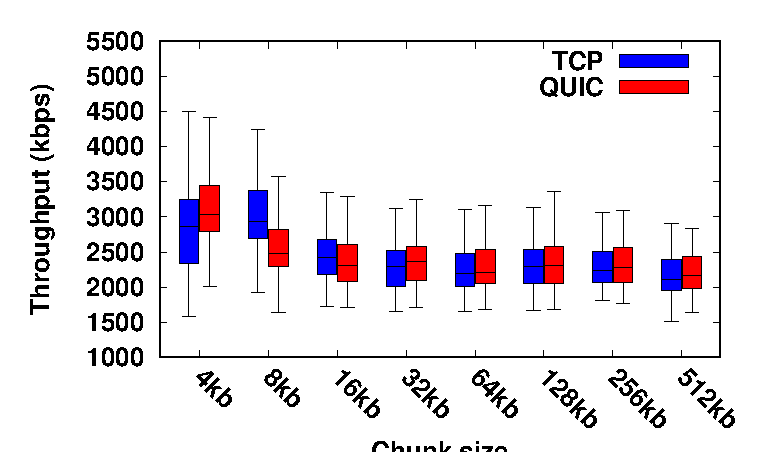
\includegraphics[width=.49\linewidth]{img/proof/uhoodS/throughput}
%	}
%	\subfloat[\label{fig:proofUhoodSWait}Response latency]{
%		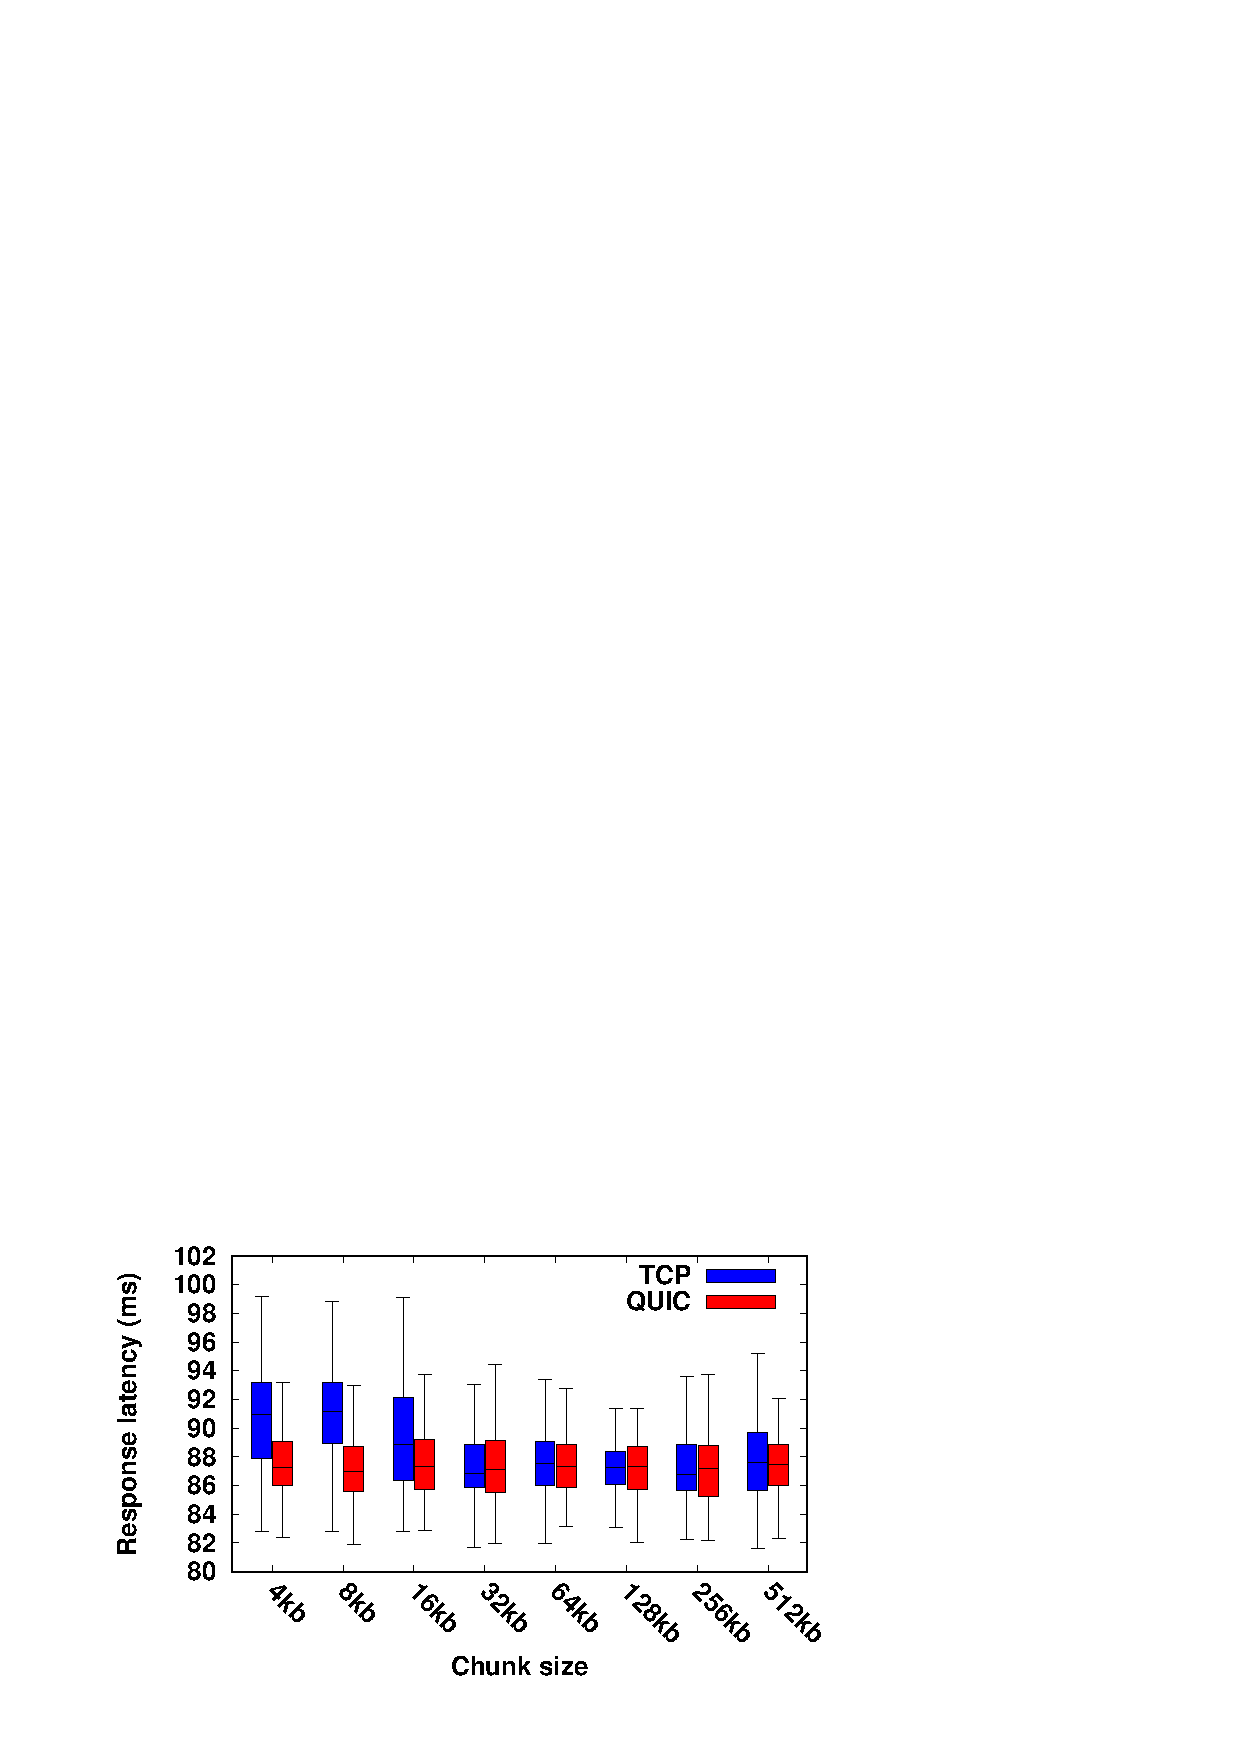
\includegraphics[width=.49\linewidth]{img/proof/uhoodS/wait}
%	}
%\end{center}
%\caption{\label{fig:proofUhoodS}Throughput and response latency observed while downloading multiple small chunks sequentially}
%\end{figure}

%\blue{
%{\bf Exp a)} We first experiment to compare the performance of HTTP over TCP and HTTP over QUIC while downloading large files. 
%}



\subsection{Exploring TCP and QUIC Connections during a Video Streaming}
%Exploring it further, we look into how the video streaming sessions are established between a DASH client and the video streaming server. 
During the dashification of a video with an embedded audio, the standard practice is to first segregate and segment the video data and the corresponding audio data, and then encode the video and the audio segments separately in their respective available encoding formats. 
%In this way, if there are $m$ and $n$ different encoding formats available for the video and the audio, respectively, then there are $m \times n$ combinations through which the video can be streamed. 
Now the DASH client creates two different HTTP streams for downloading the video segments and the corresponding audio segments. For DASH/TCP, two different TCP sockets are created between the DASH client and the server for these two HTTP streams, whereas for DASH/QUIC, both the HTTP streams are multiplexed, and the HTTP messages are exchanged over a single UDP socket. 
%This indicates that one of the major feature of streaming video connections is that two different parallel application streams are multiplexed over a single UDP socket when QUIC is used. 
This brings the next question -- how do TCP and QUIC fare for two parallel but interdependent application streams between the same client and the server?  To answer this question, we do the next experiment over the same network setup as discussed before. In this experiment, we create two HTTP streams where both the streams request for the HTTP objects (files) in parallel. The object sizes are varied from $1$MB to $8$MB. 
%In TCP, these two HTTP streams create two parallel TCP sockets, whereas in QUIC, they are multiplexed and transferred over a single UDP socket. 
We also vary the duration between two HTTP requests (called the pause time) from $500$ms to $8000$ms. 
%The pause time helps us to change the frequency of the HTTP requests -- a small pause time indicates that the requests are made very quickly, whereas a large pause time denotes that the requests are generated slowly. 


%\blue{
%{\bf Exp b)} It is an experiment to find out the responsiveness of the protocols TCP and QUIC\footnote{We should not get confuse with the head-of-the-line (HoL) blocking with responsiveness.}. Here we download a small chunk of video data repeatedly one after another for 50 times in a single session. We repeat each session three times for each protocol. Then we change the chunk size and repeat the experiment. In this experiment, we vary chunk size exponentially from 4KB to 512KB and give a pause of 500ms between two downloads.
%}

%\blue{
%We plot the observations of this experiment in Fig.~\ref{fig:proofUhoodS}. These results represent the expected performance from the QUIC compared to TCP, i.e. throughput observed by DASH player is better for QUIC than that of TCP.
%}

%\blue{
%{\bf Exp c)} Here we are trying to determine the responsive nature of two protocols when browsers are allowed to download multiple chunks parallelly. The experimental setup is the same as the previous one with few exceptions, here we vary the chunk size from 1MB to 8MB exponentially and allow parallel segment downloading. For monitoring purposes, we fixed the parallel download for each session to either 1 or 2. In this experiment, we also vary the pause duration from 500ms to 8000ms exponentially. In this experiment we also use another QUIC server implementation LightSpeed QUIC \cite{lsquic} (version 2.13.1).
%}

\begin{figure}[!ht]
	\captionsetup[subfigure]{}
	\begin{center}
		\subfloat[\label{fig:proofUhoodMThroughput2} Throughput]{
			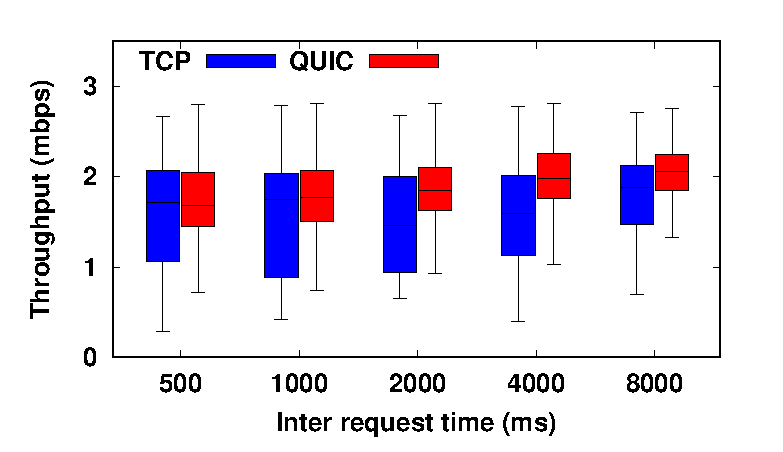
\includegraphics[width=.49\linewidth]{img/proof/uhoodM/throughput-2}
		}
		\subfloat[\label{fig:proofUhoodMWait2} Response latency ($p<0.05$ for all the instances)]{
			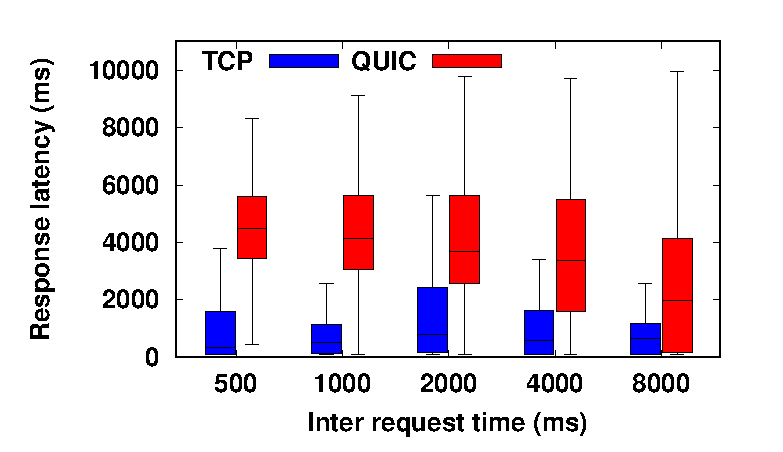
\includegraphics[width=.49\linewidth]{img/proof/uhoodM/wait-2}
		}
	\end{center}
	\caption{\label{fig:proofUhoodM}Performance of TCP and QUIC for two parallel connections}
\end{figure}


Fig.~\ref{fig:proofUhoodM} shows the observations from this experiment. The differences in throughput between QUIC and TCP is not significant; however, the response latency with QUIC is significantly higher than TCP when two parallel application streams generate HTTP requests. Further, this difference in the response latency is more prominent when the pause time is less indicating the frequency of the HTTP requests is high. This observation is very synonymous to what we observed in Fig.~\ref{fig:dashcomp}. To find out the reason for such a behavior, we see that the problem is inherited from the behavior of the socket buffers used to interface between the user-space and the kernel-space. As TCP creates two separate sockets for the two HTTP streams, each of the sockets maintains its own socket buffer. Therefore, the HTTP responses from the two streams do not interfere with each other. On the other hand, QUIC multiplexes both the streams and uses a single UDP socket having a single socket buffer. Therefore, the HTTP responses from both the streams interfere, and higher response rate at one stream affects the queuing delay for the response at the other stream. 


When DASH uses two separate HTTP streams for video and audio downloads, the stream corresponding to the video downloads has a higher data generation rate compared to the stream corresponding to the audio download. This is because the amount of video data to be downloaded is much higher compared to the amount of the audio data to be downloaded, for a fixed playback time. For DASH/TCP, the audio and the video streams use separate socket buffers, having independent queuing delay depending on their data generation rate. However, for QUIC, both the streams get multiplexed. For every playback segment, the client generates one HTTP request for the video segment and another HTTP request for the audio segment. As the video segment request is sent first, the UDP socket buffer gets filled up with the majority of the video segment data. Consequently, the data for the audio segment needs to wait until that video data gets freed up from the socket buffer. Fig.~\ref{fig:proofCompDlTime} shows an example instance of video download using QUIC, where we see that video data is served almost immediately after the request is received at the server. However, the audio data has to wait in the queue (the red timeline) before it gets served. This problem is not there in TCP as the fairness property of TCP flow and congestion control serves both the socket buffers in a fair way. So, the audio data does not experience this high response latency. Fig.~\ref{fig:proofCompAVLatency} shows the distributions of the response latency for the audio and video streams separately. We see that the distributions of the response latency for the video streams are similar for QUIC and TCP. However, the audio streams at QUIC experiences a much higher latency compared to TCP. 


\begin{figure}[!ht]
	\captionsetup[subfigure]{}
	\begin{center}
   		\subfloat[\label{fig:proofCompDlTime} Video/Audio downloads over QUIC]{
   			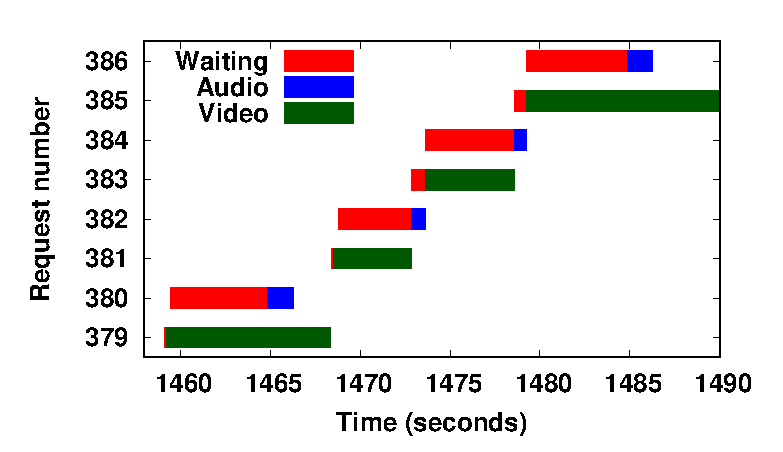
\includegraphics[width=.45\linewidth]{img/proof/comp/ls}
   		}
           		\hfill
		\subfloat[\label{fig:proofCompAVLatency} Response latency for audio and video]{
			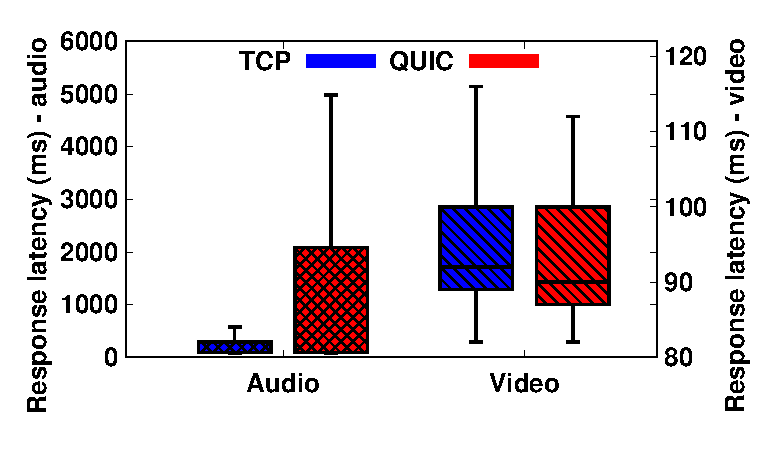
\includegraphics[width=.45\linewidth]{img/proof/comp/avwait}
		}
	\end{center}
	\label{fig:dashcompres}
	\caption{TCP and QUIC response latency during video and audio downloads over separate streams}
\end{figure}


\subsection{Summary}
We observe that during parallel downloads of audio and video streams, QUIC multiplexing affects the response latency of the audio streams. This observation also tallies with the observation made in~\cite{kakhki2019taking} which states that multiplexing objects from parallel streams affect the latency of individual objects. This latency is inevitable because of multiplexing multiple objects over a single UDP queue, whereas the final video playback depends on successful download of both the video and the audio segments. Interestingly, the throughput calculation used in DASH does not consider this response latency, resulting in a mismatch between the expected throughput and the actual download time of the segments after a request is sent. There might not be a direct solution to this problem as DASH is unaware about such behaviors of the underlying data transmission protocol, whereas QUIC is unaware about the dependency between the audio and the video streams for successful streaming of the video. A further analysis and protocol enhancement is required in this space for making ABRs work perfectly on top of QUIC.   


%\blue{
%However, there might not be a direct solution to the above problem, as by the nature of the segment size for the audio and the video requests, it is likely that more video segment requests/responses will be generated than audio segment requests/responses for a fixed playback duration. Therefore, a fair scheduling of the requests/responses for the audio and the video streams might not help in solving the problem, as the audio requests/responses may still experience the queuing delay based on the frequency of the video requests/responses. Further, the DASH client is unaware about such behavior of the underlying network protocols, and it generates the requests independently. The QUIC is also unaware about this dependency between the two streams, and therefore, it does not treat the requests from the two streams accordingly, resulting in high response latency for some requests and thus degrading the video QoE.  
%}

%\blue{
%\textit{Discussion:}
%With thorough experiments, it is clear that QUIC has issues with responsiveness during parallel connections. However, we are not sure whether it is a problem with the browser or server implementation. We even run under the hood experiments with another QUIC server implementation LightSpeed-QUIC (LS-QUIC) \cite{lsquic} and find a similar result.  We are not putting any plot regarding this as it does not contain any new information. So, we can safely conclude that it is not an implementation problem rather a system problem.
%}

%\blue{
%It is clear from Fig.~\ref{fig:proofUhoodS} and Fig.~\ref{fig:proofUhoodM} that both the protocols have longer response latencies during parallel downloads compared to the sequential downloads. However, the response latency for QUIC is double that of the TCP. It indicates that there are some problems with one or more queues at the sender side and the receiver side as well. In the case of HTTP over TCP, there is a dedicated TCP connection between source and destination for each HTTP request-response. Each TCP connections have an independent sender queue as well as a receiver queue in the transport layer of the kernel. By default, TCP connections are incredibly fair to a new and existing connection. Any new TCP connection can start as soon as a user wants to connect to the server without any interference from other ongoing TCP connections. However, it has to wait if the interface queue is full. It is the reason there is an increase in the response latency for parallel connections as the first connection has filled the interface queue, and the second connection has to go through the queue.
%}
%
%\blue{
%On the other hand, QUIC multiplexes all the HTTP connections over a single UDP socket. In a Linux system, the UDP socket has a sender buffer to store the packet received from the application and forward it to the lower layer. As QUIC usage a single UDP socket, every packet it transmits, needs to go through the transport layer buffer to reach the network. When there is a single QUIC stream in the system, and it has enough data to send, it consumes the entire UDP socket buffer. At this time, if a new QUIC stream enters the system, it can not reach the network unless previous UDP packets reach the network. The QUIC cannot do anything about it. It can cause increase response latency significantly for the second HTTP request. There is a way to solve this problem by reducing the system-wide UDP buffer. However, The configuration to change the amount of buffer is shared between the receiver and the sender side of all the UDP sockets, so we can not change one side (i.e., sender side) without affecting the other. It will cause a massive number of UDP packet drop as there is no space in the buffer to store the newly arrived packet, which affects the QUIC's throughput.
%}
%
%
%%\blue{However, we don't what is the specific reason behind these difference. So, we dig more to understand the communication behaviour that are visible to the ABR. ABR get these information from DASHJS and DASHJS get them by looking at the AJAX calls. To monitor these AJAX call we design a small chrome extension using chrome-webRequest API \cite{webrequest}. From the extension, we retrieve details like response latency, goodput for each and every AJAX call by the DASHJS.}


%\begin{figure}
%	\begin{center}
%			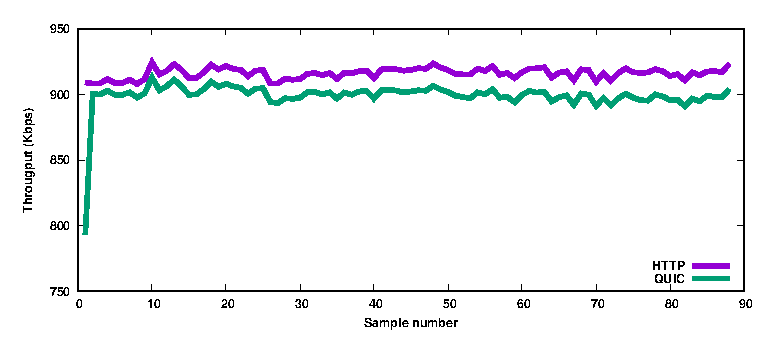
\includegraphics[width=.95\linewidth]{img/bandwidthComp}		
%	\end{center}
%	\caption{\label{fig:bandwithcomp}Observered bandwidth by the client}
%\end{figure}

%\begin{figure}
%	\begin{center}
%		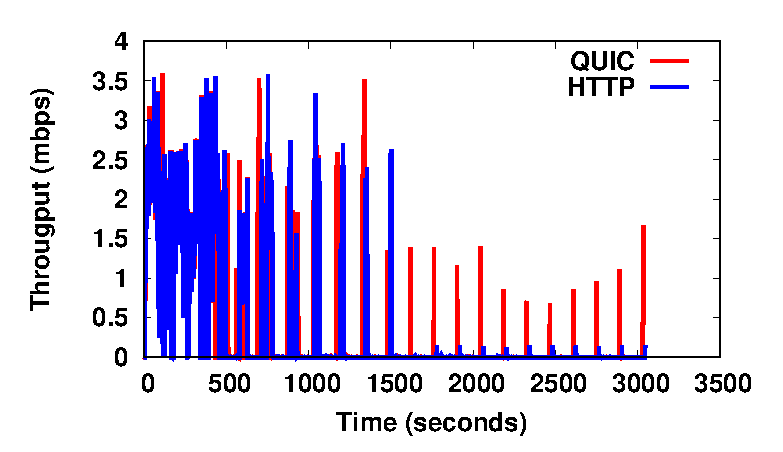
\includegraphics[width=.85\linewidth]{img/newexp/throughput.eps}
%	\end{center}
%	\caption{\label{fig:bandwithcomp}Observed bandwidth (link throughput) by the client}
%\end{figure}
%\subsection{Discussion -- Why TCP Performs Better}
%\blue{
%In our thorough experiments with a wide variety of ABRs, we find that none of the ABR performs at per TCP while using QUIC as the transport protocol. While digging deep, we find that QUIC suffers from low responsiveness problems. We also see that this responsiveness only matters when there are simultaneous downloading going on. It creates a problem for DASH.JS because DASH.JS sometimes try to download audio and video chunks simultaneously. As DASH.JS does not include the response latency during the measurement of the throughput, it leads ABR to take the incorrect decision of quality, which leads to rebuffering.
%}
%
%\blue{
%Almost all the ABR techniques directly or indirectly depend on the observed throughput; however, none of the existing ABRs consider the response latency directly. Buffer based ABR techniques indirectly consider the response latency by looking at the buffer changes. However, this not accurate either.
%}

\begin{comment}
Our thorough experiments over a wide range of ABR techniques indicate that the existing ABR techniques are more compatible with HTTP/TCP than QUIC. Almost all the ABR techniques are directly or indirectly dependent on the link bandwidth (or throughput) perceived by the client. In our experimental setup, the link bandwidth has been regulated at the traffic shaper. Therefore, we see that the client observe similar link throughput patterns for both TCP and QUIC; however, the client-perceived instantaneous throughput is marginally higher with TCP compared to QUIC (a difference of $\approx{40}$kbps). 

Typically QUIC provides a better end-to-end performance compared to TCP over a high-loss high-latency link~\cite{langley2017quic}. However, for general network traces like the ones we used in this experiment, we observe that packet loss and high latency are typically instantaneous and are not long-term factors. Further, video streaming sessions with QUIC are in-general long flows with a single end-to-end connection, whereas TCP uses separate connections (short-lived flows) for each data segment download. As a consequence, TCP spends majority of the time in the slow-start phase, whereas QUIC remains in the congestion avoidance phase. As TCP increases the bandwidth exponentially at the slow-start, the instantaneous throughput with TCP gets higher than that of QUIC, although the network condition remains the same. As shown in Fig.~\ref{fig:bandwithcomp} for an example of a sample video streaming, HTTP/TCP aggressively downloads the video segments within half of the video-playback duration, whereas QUIC maintains a steady throughput during the video download sessions throughout the playback duration by maintaining a single end-to-end connection. As a consequence, the instantaneous link throughput observed by the client is more for HTTP/TCP compared to QUIC. As mentioned by the authors of Pensieve~\cite{mao2017neural}, a small change in the client-observed bandwidth can significantly impact the QoE performance, which we observe here. 

Indeed, the current ABR techniques are more sensitive towards instantaneous throughput rather than long-term throughput. As QUIC provides a steady bandwidth during the entire playback duration by maintaining a single connection, the video playback smoothness is better with QUIC (Fig.~\ref{fig:averageQualityVariation_n}). However, a high value in the instantaneous throughput in TCP increases the video quality level (Fig.~\ref{fig:averageQuality_n}); further, the quality levels are quickly adapted based on the client-perceived throughput, which reduces the rebuffering as we observe in Fig.~\ref{fig:RebufferTime_n}. This indicates that the existing ABR techniques are more sensitive to sudden fluctuations in the link throughput as they primarily look into the instantaneous throughput behavior, whereas QUIC focuses on providing a steady throughput for the entire duration of a long flow. 
%Therefore, the ABR techniques over QUIC need to focus on the prediction of long-term link throughput rather than being aggressive towards the instantaneous link conditions.  
%
%In summary, we observe that the nature of current ABR techniques are more compatible with HTTP/TCP, and new ABR techniques need to be designed to get the best out of QUIC. More specifically, 


%While we plot the quality of experience to compare the performance of HTTP and QUIC, we found that QUIC does under perform for both linear and logarithmic QoE measurement. QUIC is under performing almost all the metric except startup delay. startup delay using QUIC is lesser than HTTP.  It is a major drawback for QUIC in contrast of DASH based video streaming. Although Google claims in \cite{QUIC-2017} that QUIC performs well for video streaming, it is not. This is a experiment with simple DASH based player without any specific modification to the DASH ABR algorithm for QUIC.
\end{comment}



%\begin{figure}
%	\captionsetup[subfigure]{}
%	\begin{center}
%		\subfloat[\label{fig:StartupDelay_box}]{
%			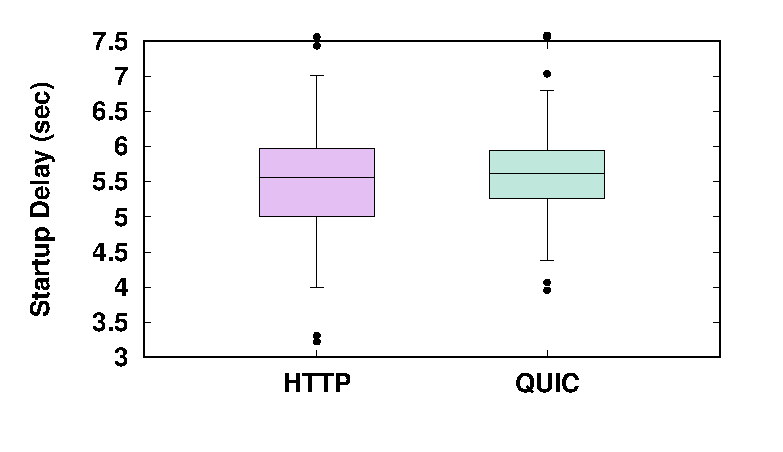
\includegraphics[width=.49\linewidth]{img/exp/SD_box}
%		}
%		\subfloat[\label{fig:StartupDelay_cmf}]{
%			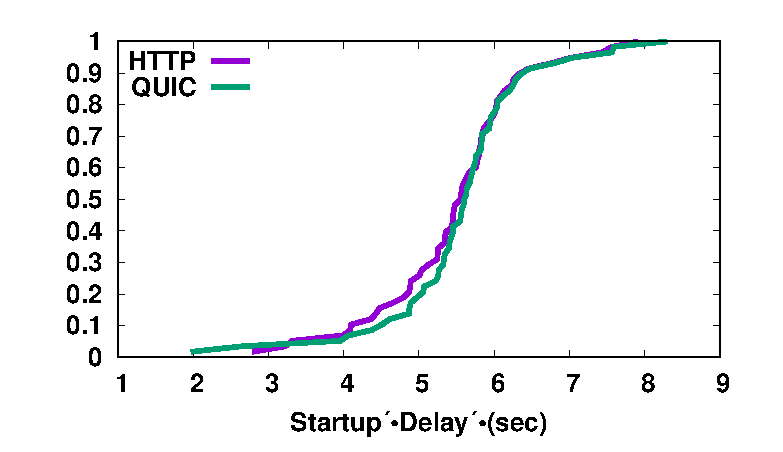
\includegraphics[width=.49\linewidth]{img/exp/SD_cmf}
%		}
%	\end{center}
%	\caption{\label{fig:StartupDelay}Startup Delay (RanksumsResult(statistic=-0.5438835568896925, pvalue=0.5865216048375494))}
%\end{figure}
% (RanksumsResult(statistic=-0.5438835568896925, pvalue=0.5865216048375494))

%From our previous experiment, it is clear that QUIC does not performs as good as HTTP under the similar environment. Although at this point we are not sure why QUIC is under performing, it have something to do with the DASH observed bandwidth, because no external parameter have been changed during experiments. To confirm if it the bandwidth provided by the QUIC and TCP, we perform few test to understand the DASH observed bandwidth. In this experiment, we downloaded multiple files from the server using javascript and measured the bandwidth observed by the javascript itself. The result is plotted in Fig.~\ref{fig:bandwithcomp}. From this plot, it is clear that the bandwidth achieved by crude HTTP is slighlty higher that the QUIC. However, this slight change can in observed bandwidth can deprive the entire bitrate in case of DASH based video streaming as suggested by \cite{pensiev2017}. The reason QUIC is underperforming slightly is the short live connection. In case of QUIC, it is maintaining a long lived connection between server and the browser. But, in case of TCP, browser needs to make a new connection for each and every data download. As data size is very small, TCP never exited from slow-start phase. In slow-start phase, congestion window can grows exponentially which helps TCP achieve slightly better bandwidth. However, QUIC keep continuous connection, which spent most of the time in congestion avoidance phase.


